% ch05-forward-fixpoint.tex — Forward Chaining with θ and Fixpoint
% Shows G₀ → G₁ → G₂ → fixpoint with substitution annotations.
% Pedagogical purpose: make the iterative rule application mechanism concrete.
\documentclass[tikz,border=5pt]{standalone}
\usepackage{fontspec}
\setmainfont{Times New Roman}
\usepackage{unicode-math}
\setmathfont{Cambria Math}
\usetikzlibrary{shapes.geometric,shapes.misc,positioning,fit,backgrounds,arrows.meta}

\begin{document}
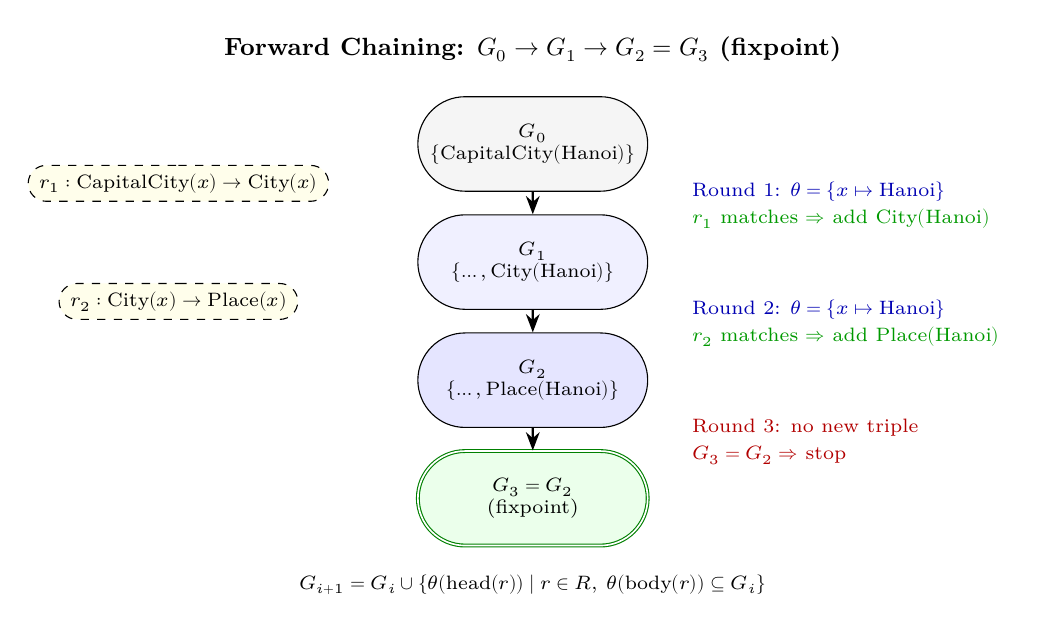
\begin{tikzpicture}[
  round/.style={rounded rectangle,draw,minimum width=3.2cm,minimum height=1.2cm,
                font=\scriptsize,align=center,inner sep=4pt},
  rulebox/.style={rounded rectangle,draw,dashed,font=\scriptsize,inner sep=3pt,
                  fill=yellow!8,minimum width=2.8cm},
  arr/.style={->,>=Stealth,thick},
  theta/.style={font=\scriptsize,text=blue!70!black},
  newfact/.style={font=\scriptsize,text=green!60!black},
  title/.style={font=\small\bfseries},
]

% Title
\node[title] at (0,4.2) {Forward Chaining: $G_0 \to G_1 \to G_2 = G_3$ (fixpoint)};

% Rules annotation
\node[rulebox] at (-4.5,2.5) {$r_1: \mathrm{CapitalCity}(x) \to \mathrm{City}(x)$};
\node[rulebox] at (-4.5,1.0) {$r_2: \mathrm{City}(x) \to \mathrm{Place}(x)$};

% G0
\node[round,fill=gray!8] (G0) at (0,3.0) {$G_0$\\$\{\mathrm{CapitalCity}(\mathrm{Hanoi})\}$};

% G1
\node[round,fill=blue!6] (G1) at (0,1.5) {$G_1$\\$\{\ldots, \mathrm{City}(\mathrm{Hanoi})\}$};

% G2
\node[round,fill=blue!10] (G2) at (0,0.0) {$G_2$\\$\{\ldots, \mathrm{Place}(\mathrm{Hanoi})\}$};

% G3 = G2 (fixpoint)
\node[round,fill=green!8,draw=green!50!black,double] (G3) at (0,-1.5) {$G_3 = G_2$\\(fixpoint)};

% Arrows between rounds
\draw[arr] (G0) -- (G1);
\draw[arr] (G1) -- (G2);
\draw[arr] (G2) -- (G3);

% Round labels with θ
\node[theta,anchor=west] at (1.9,2.4)
  {Round 1: $\theta = \{x \mapsto \mathrm{Hanoi}\}$};
\node[newfact,anchor=west] at (1.9,2.05)
  {$r_1$ matches $\Rightarrow$ add $\mathrm{City}(\mathrm{Hanoi})$};

\node[theta,anchor=west] at (1.9,0.9)
  {Round 2: $\theta = \{x \mapsto \mathrm{Hanoi}\}$};
\node[newfact,anchor=west] at (1.9,0.55)
  {$r_2$ matches $\Rightarrow$ add $\mathrm{Place}(\mathrm{Hanoi})$};

\node[font=\scriptsize,text=red!70!black,anchor=west] at (1.9,-0.6)
  {Round 3: no new triple};
\node[font=\scriptsize,text=red!70!black,anchor=west] at (1.9,-0.95)
  {$G_3 = G_2 \Rightarrow$ stop};

% Formula at bottom
\node[font=\scriptsize,align=center] at (0,-2.6)
  {$G_{i+1} = G_i \cup \{ \theta(\mathrm{head}(r)) \mid r \in R,\; \theta(\mathrm{body}(r)) \subseteq G_i \}$};

\end{tikzpicture}
\end{document}
